\chapter{On logical correspondence}

In Part 1, we defined \sls, a logical framework of substructural
logical specifications. For the purposes of this thesis, we are
primarily interested in using \sls~as a framework for specifying the
operational semantics of programming languages, especially stateful
and concurrent programming languages. This is not a new idea: one of
the original case studies on CLF specification described the semantics
of Concurrent ML \cite{cervesato02concurrent} in a specification style
termed {\it substructural operational semantics}, or SSOS, by Pfenning
\cite{pfenning04substructural}. The general idea of representing the
intermediate states of a computation as contexts in substructural
logic dates back to Miller \cite{miller92pi} and his Ph.D. student
Chirimar \cite{chirimar95proof}, who encoded the intermediate states
of a $\pi$-calculus and of a low-level RISC machine (respectively) as
contexts in focused classical linear logic.

However, the design space of substructural operational semantics is
extremely rich. In order to make sense of the design space, it is
helpful to have design principles that allow us to both {\it classify}
different styles of presentation and {\it predict} what style(s) we
should adopt based on what our goals are. In this thesis, I propose a
classification scheme for substructural operational semantics based on
the consideration of three major specification styles.  Each of these
styles is more expressive than the last.

\begin{itemize}
\item The {\it natural semantics}, or big-step operational semantics,
  is an existing and well-known specification style (and not a
  substructural operational semantics). It is convenient for the
  specification of pure programming languages.

\item The {\it ordered abstract machine semantics} is a generalization
  of abstract machine semantics that can be naturally specified in
  \sls; this specification style naturally handles stateful and
  parallel programming language features
  \cite{pfenning09substructural}.

\item The {\it destination-passing semantics} is the style of
  substructural operational semantics first explored in CLF by
  Cervesato et al.~\cite{cervesato02concurrent}. It allows for the
  natural specification of features that incorporate synchronous
  communication and non-local transfer of control. Destination-passing
  semantics are classified into two subspecies: those with linear
  continuations and those with persistent continuations. Persistent
  continuations are necessary to give a substructural operational
  semantics to languages with first-class continuations.
\end{itemize}


\begin{figure}
\begin{center}
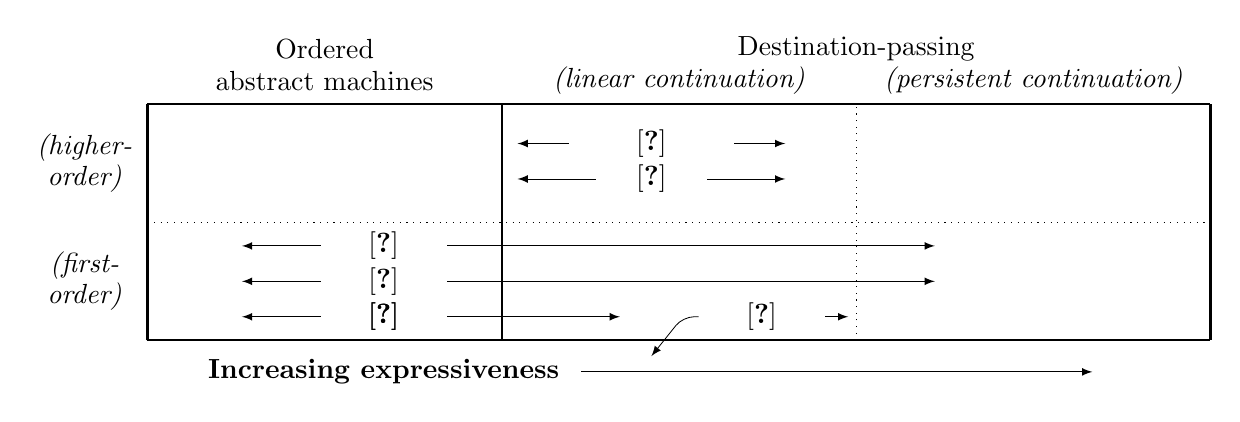
\begin{tikzpicture} 
\draw[thick](0cm,0cm) -- (0cm,3cm);
\draw (2.25,3.7) node{Ordered};
\draw (2.25,3.3) node{abstract machines};
%
\draw[thick](4.5cm,0cm) -- (4.5cm,3cm);
\draw (9,3.7) node{Destination-passing};
\draw (6.75,3.3) node{\it (linear continuation)};
%
\draw[dotted](9cm,0cm) -- (9cm,3cm);
\draw (11.25,3.3) node{\it (persistent continuation)};
%
\draw[thick](13.5cm,0cm) -- (13.5cm,3cm);
%
\draw[thick](0,0) -- (13.5,0);
\draw[dotted] (0,1.5) -- (13.5,1.5);
\draw[thick](0,3) -- (13.5,3);
%
\draw (-.8,2.45) node{\it (higher-};
\draw (-.8,2.05) node{\it order)};
%
\draw (-.8,0.95) node{\it (first-};
\draw (-.8,0.55) node{\it order)};
%
\draw (3,1.2) node{\cite{pfenning04substructural}};
\draw (3,.75) node{\cite{pfenning09substructural}};
\draw (3,.3) node{\cite{simmons11logical}};
\draw (3,.3) node{\cite{simmons11logical}};
\draw (7.8,.3) node{\cite{pfenning12substructural}};
\draw (6.4,2.5) node{\cite{cervesato02concurrent}};
\draw (6.4,2.05) node{\cite{schacknielsen07induction}};
\draw (3,-.4) node{\bf Increasing expressiveness};
%
\pgfsetarrowsstart{latex} 
\pgfsetlinewidth{.3pt} 
\pgfusepath{stroke} 
\draw (1.2,1.2) -- (2.2,1.2);
\draw (10,1.2) -- (3.8,1.2);
\draw (1.2,.75) -- (2.2,.75);
\draw (10,.75) -- (3.8,.75);
\draw (1.2,.3) -- (2.2,.3);
\draw (6,.3) -- (3.8,.3);
\draw[rounded corners=4pt] (6.4,-.2) -- (6.8,.3) -- (7,.3);
\draw (8.9,.3) -- (8.6,.3);
\draw (4.7,2.5) -- (5.35,2.5);
\draw (4.7,2.05) -- (5.7,2.05);
\draw (8.1,2.5) -- (7.45,2.5);
\draw (8.1,2.05) -- (7.1,2.05);
%
\draw (12,-.4) -- (5.5,-.4);
\end{tikzpicture} 
\end{center}
\caption{Classification of existing work on SSOS specifications.}
\label{fig:class-prevwork}
\end{figure}

This classification of substructural operational semantics is
illustrated graphcially in Figure~\ref{fig:class-prevwork}. Existing
published work on substructural operational semantics specifications
is placed in the figure, with arrows indicating the range of styles
that are considered. With the possible exception of certain aspects of
the SSOS presentation in Pfenning's course notes
\cite{pfenning12substructural}, the taxonomy described above neatly
captures previous work. 

The statement that each specification style is strictly more
expressive than the last is formal: there are automatic and
provably-correct transformations from the expressive styles (natural
semantics and ordered abstract machines) to the more expressive
formalisms (ordered abstract machines and destination-passing).  The
investigation of provably-correct transformations on
\sls~specifications is therefore the means by which we classify of
SSOS semantics. We call this methadology the {\it logical
  correspondance}, and it is the focus of this portion of the thesis,
which justifies the following argument:

\begin{quote} 
  {\bf Thesis (part 2):} A logical framework based on forward
  reasoning in substructural logic supports many styles of programming
  language specification. These styles can be formally classified and
  connected by considering general transformations on logical
  specifications. 
 
  Generally applicable transformations on logical
  specifications are also useful for deriving manifestly correct
  program analyses from those operational semantics specifications.
\end{quote} 

\noindent
In this introductory chapter, we will outline our use of logical
correspondence and connect it to previous work.

\section{Logical correspondence}

As stated above, we will primarily discuss and connect three different
styles that are used specifying the operational semantics of
programming languages. Natural semantics is a high-level, declarative
style of specification. For illustration, the call-by-value natural
semantics for the untyped lambda calculus is comprised of two rules:
\[
\infer[{\sf ev/lam}]
{\lambda x. e \Downarrow \lambda x. e \mathstrut}
{}
\quad
\infer[{\sf ev/app}]
{e_1\,e_2 \Downarrow v \mathstrut}
{e_1 \Downarrow \lambda x.e
 &
 e_2 \Downarrow v_2
 &
 [v_2/x]e \Downarrow v \mathstrut}
\]
This inductive definition assigns meaning to all the terminating
expressions in the lambda calculus. However, natural semantics are not
{\it operational} semantics, except in the very loose sense that they
are {\it moded} in the sense of Section~\ref{sec:framework-modes}: we
can think of the $e$ in $e \Downarrow v$ as being an input and the $v$
as being output. The order of evaluation is unspecified, however.  In
rule ${\sf ev/app}$, the subexpressions $e_1$ and $e_2$ can be
evaluated to values in either order and can even be evaluated in
parallel.

We turn natural semantics into ordered abstract mahcines by
a transformation called {\it operationalization}, and turn ordered
abstract machine specifications into destination-passing
specifications by a transformation called {\it destination-adding}.
Destination-passing specifications can then be transformed into a
collecting semantics by the simple transformation of {\it
  abstraction}, after which they can be further abstracted to obtain
program analyses like control flow analysis. These major
transformations are presented graphcially in
Figure~\ref{fig:class-transform}.

\begin{figure}
\begin{center}
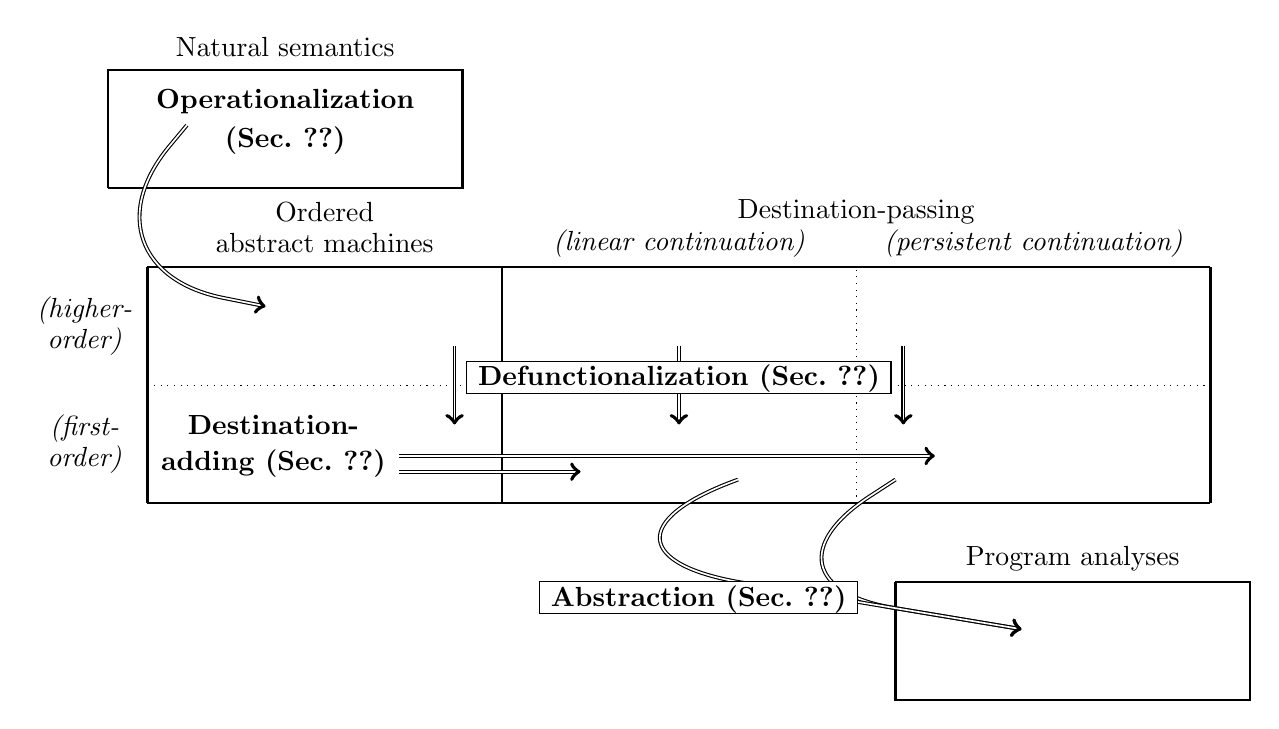
\begin{tikzpicture}
\draw (1.75,5.8) node{Natural semantics};
\draw[thick](-.5cm,4cm) -- (-.5cm,5.5cm) -- (4cm,5.5cm) 
  -- (4cm,4cm) -- (-.5cm,4cm);
%
\draw (11.75,-.7) node{Program analyses};
\draw[thick](9.5cm,-1cm) -- (9.5cm,-2.5cm) -- (14cm,-2.5cm) 
  -- (14cm,-1cm) -- (9.5cm,-1cm);
%
\draw[thick](0cm,0cm) -- (0cm,3cm);
\draw (2.25,3.7) node{Ordered};
\draw (2.25,3.3) node{abstract machines};
%
\draw[thick](4.5cm,0cm) -- (4.5cm,3cm);
\draw (9,3.7) node{Destination-passing};
\draw (6.75,3.3) node{\it (linear continuation)};
%
\draw[dotted](9cm,0cm) -- (9cm,3cm);
\draw (11.25,3.3) node{\it (persistent continuation)};
%
\draw[thick](13.5cm,0cm) -- (13.5cm,3cm);
%
\draw[thick](0,0) -- (13.5,0);
\draw[dotted] (0,1.5) -- (13.5,1.5);
\draw[thick](0,3) -- (13.5,3);
%
\draw (-.8,2.45) node{\it (higher-};
\draw (-.8,2.05) node{\it order)};
%
\draw (-.8,0.95) node{\it (first-};
\draw (-.8,0.55) node{\it order)};
%
\draw[double,->] (3.9,2) -- (3.9,1);
\draw[double,->] (6.75,2) -- (6.75,1);
\draw[double,->] (9.6,2) -- (9.6,1);
\draw (6.75,1.6) node {\fboxsep=0pt\fbox{\colorbox{white}{\rule[-0.5ex]{0em}{2.5ex}\bf ~Defunctionalization~(Sec.~\ref{sec:defunctionalization})~}}};
%
\draw (1.75,5.1) node {\bf Operationalization};
\draw (1.75,4.6) node {\bf (Sec.~\ref{sec:operationalization})~};
\draw[double,->,rounded corners=2cm] (.5,4.8) -- (-1,3) -- (1.5,2.5);
%
\draw (1.6,1) node {\bf Destination-};
\draw (1.6,.5) node {\bf adding (Sec.~\ref{sec:destination-adding})};
\draw[double,->] (3.2,.6) -- (10,.6);
\draw[double,->] (3.2,.4) -- (5.5,.4);
%
\draw[double,->,rounded corners=2cm] (9.5,.3) -- (7.5,-1) -- (11.1,-1.6);
\draw[double,->,rounded corners=2.5cm] (7.5,.3) -- (5.1,-.6) -- (11.1,-1.6);
\draw (7,-1.2) node {\fboxsep=0pt\fbox{\colorbox{white}{\rule[-0.5ex]{0em}{2.5ex}\bf ~Abstraction~(Sec.~\ref{sec:abstraction})~}}};
\end{tikzpicture} 
\end{center}
\caption{Major transformations on \sls~specifications.}
\label{fig:class-transform}
\end{figure}

There are many other smaller design decisions that can be made in the
creation of a substructural operational semantcs. Only one is
graphcially represented in
Figures~\ref{fig:class-prevwork}~and~\ref{fig:class-transform}, the
distinction between {\it higher-order} or {\it first-order}
specifications. This distinction applies to all concurrent
\sls~specifications, not just those that specify substructural
operational semantics. First-order
specifications are like rewriting rules $\left( p_1 \fuse \ldots \fuse
  p_n \lefti \{ q_1 \fuse \ldots \fuse q_m \} \right)$, where the head
of the rule $\{ q_1 \fuse \ldots \fuse q_m \}$ contains only atomic
propositions. Higher-order \sls~specifications, on the other hand,
contain {\it rules} in the conclusions of rules; when the rule fires,
the resulting process state contains the rule. An example is given 
in Figure~\ref{fig:ho-evo-ex}.
Order matters in higher-order process states: $\left(x{:}\susp{\sf p1(c)}, ~
y{:}\istrue{\left( {\sf p1(c)} \lefti \{ {\sf p2(c)} \} \right)}\right)
\leadsto \left(z{:}\susp{\sf p2(c)}\right)$, whereas 
$\left(y{:}\istrue{\left( {\sf p1(c)} \lefti \{ {\sf p2(c)} \} \right)},~
x{:}\susp{\sf p1(c)}\right)
\not \leadsto$. 
%
The choice of higher-order versus first-order specification does not
impact expressiveness, but it does influence our ability to read
specifications (opinions differ as to which style is clearer) and 
the ways we reason about them.

\begin{figure}
\begin{align*}
x_1{:}\susp{{\sf p2}({\sf c})}, ~~
x_2{:}\susp{{\sf p1}({\sf c})}, ~~
x_3{:}\istrue{(\forall x.\,{\sf p_1}(x) 
                \lefti \{ {\sf p_2}(x) \lefti \{ {\sf p_3}(x) \} \})}, ~~
x_4{:}\istrue{({\sf p3}({\sf c}) \lefti \{ {\sf p_4} \})} & \\
\leadsto ~~~ 
x_1{:}\susp{{\sf p2}({\sf c})}, ~~
x_5{:}\istrue{({\sf p_2}({\sf c}) \lefti \{ {\sf p_3}({\sf c}) \})}, ~~
x_4{:}\istrue{({\sf p3}({\sf c}) \lefti \{ {\sf p_4} \})} & \\
\leadsto ~~~ 
x_6{:}\susp{{\sf p3}({\sf c})}, ~~
x_4{:}\istrue{({\sf p3}({\sf c}) \lefti \{ {\sf p_4} \})} & \\
\leadsto ~~~ 
x_7{:}\susp{{\sf p_4}} & 
\end{align*}
\caption{Evolution of a higher-order \sls~process state (${\sf p1}$, ${\sf
  p2}$ and ${\sf p3}$ are all ordered atomic propositions).}
\label{fig:ho-evo-ex}
\end{figure}

Other distinctions between \sls~specifications can also be understood
in terms of nondeterminstic choices that can be made by the various
transformations we consider: for instance, the operationalization
transformation can produce ordered abstract machines that evaluate
subcomputations in parallel or in sequence or not, and the
destination-adding transformation can make continuations either linear
or persistent. The existance of these nondeterminstic choices have two
important consequences. First, it is generally the case that one source
specification (a natural semantics or an ordered abstract machine
specification) can give rise to several different target
specifications (ordered abstract machine specificationss or
destination-passing specifications). The correctness of the
transformation also acts as a simple proof of the equivalence of the
several target specifications.

The other interesting consequence of nondeterministic choices is the
different options give us a rigorous vocabulary for describing choices
that otherwise seem ad-hoc. An example of this can be found in the
paper that introduced the destination-adding and abstraction
transformations \cite{simmons11logical}. In that article, we had to
motivate an ad-hoc change to the usual abstract machine semantics. In
this thesis, by the time we encounter a similar specification in
Chapter 8, we will be able to see that this distinction corresponds to
the choice of whether or not tail-recursion optimization is performed
during proof search.

\section{Related work}

This part of the thesis document document draws from many different
sources of inspiration. 

\subsection{Partiality in proof search}

The operationalization transformation is inspired by the threatment of
the operational semantics of LF in Tom Murphy VII's thesis
\cite{murphy08modal}. In that thesis, he describes a natural semantics
for Lambda 5, a distributed programming language, and then wanted to
interpret that natural semantics as an {\it operational} semantics for
Lambda 5. By modifying the checks that Twelf performs with a special
purpose partiality directive, he was able to check that moded proof
search for proofs in his natural semantics would never fail and never
backtrack, though it might diverge. This check amounted to a proof of
safety (progress and preservation) for his natural semantics. 

\subsection{A coinductive interpretation}

\subsection{Transformation on specifications}

From the other direction,
Hannan and Miller \cite{hannan92operational} and Ager
\cite{ager04natural} have also proposed the idea of operationalizing
natural semantics specifications as abstract machines by provably
correct and general transformations on logical specifications (in the
case of Hannan and Miller) or on the special-purpose framework of
L-attributed natural semantics (in the case of Ager). A major
difference in this case is that both lines of work result in {\it
  deductive} specifications of abstract machines. Our translation into
concurrent specifications has the advantage of exploiting parallelism,
as demonstrated in Section~\ref{sec:trans-par} below, and also opens
up specifications to the modular inclusion of stateful and concurrent
features, as we will discuss in
Section~\ref{sec:richer-ordered-abstract}.

\subsection{The functional correspondence}

The potential design space of substructural operational semantics is
quite large.  In order to make sense of this space, it is helpful to
have design principles that allow us to both {\it classify} different
styles of presentation and {\it predict} what style(s) we should adopt
based on what our goals are. I propose that different styles of
\sls~specification can be productively classified in terms of the
transformations that turn one classification style into another. Most
transformations will not have inverses, so this methodology gives us a
formal notion of which styles are more expressive than others.
Considering logical transformations also can lower the cost of
mis-prediction. If one begins a development in an overly-restrictive
style, the development can be transformed into a more expressive style
by an automatic transformation.

The organizing principle that we put forth in this chapter and the
next one is called the {\it logical correspondence}, by analogy with
the {\it functional correspondence} of Ager, Danvy, Midtgaard, and
others~\cite{ager03functional,ager04functional,ager05functional,
  danvy08defunctionalized,danvy12interderiving} in which existing styles of specification
are related to each other by way of transformations on functional
programs. It is not our goal here to detail the parallels between the
logical and functional correspondence; rather, we want to emphasize
the use of the logical correspondence to relate substructural
operational to each other and to the natural semantics.

Natural semantics specifications are not substructural operational
specifications: the LF encodings of such specifications can generally
be done just as well in LF or in the purely-persistent, non-modal
fragment of \sls. It is not my purpose to advocate for natural
semantics; recall that natural semantics were used to illustrate
problems with {\it non}-modularity in language specification in
Section~\ref{sec:modularnonmodular}. Instead, we are trying to

The examples given in the previous section have given so far all deal
with call-by-value semantics for the untyped lambda calculus, which
has the property that any expression will either evaluate forever or
will eventually evaluate to a value $\lambda x. e$. One of the
advantages of the operationalization transformation, however, is that
it allows us to

de-mystify operational semantics by showing that they are 

Instead, we are formalizing the
intuition that, on a ad-hoc basis, it is clear how t 

But natural semantics are
quite standard and widely understood, and 


 and are easy to talk about
using 

reasonably illustrate


To finish the presentation of the operationalization transformation,
we give a few more examples, which 

\subsection{}


\section{Expressiveness and modular extension}

The functional correspondance is largely concerned with the 

\sls~is very
The potential design space of substructural operational semantics is
quite large. 

I propose that different styles of
\sls~specification can be productively classified in terms of the
transformations that turn one classification style into another. Most
transformations will not have inverses, so this methodology gives us a
formal notion of which styles are more expressive than others.
Considering logical transformations also can lower the cost of
mis-prediction. If one begins a development in an overly-restrictive
style, the development can be transformed into a more expressive style
by an automatic transformation.


\begin{center}
{\it Theme:}

\medskip

A logical framework based on forward reasoning in substructural logic
supports many styles of programming language specification. These
styles can be formally classified and connected by considering
generally applicable transformations on logical
specifications. Generally applicable transformations on logical
specifications are also useful for derive program analyses from those
operational semantics specifications.
\end{center}


